\section[Cote 156-9 : un spatios fini qui n'est pas orthomodulaire]{Cote 156-9 : un spatios fini qui n'est pas orthomodulaire\protect\verifie[\leanblobmain]{Folder156_9}}\label{sec:156-9}

La cote 156-9, chapitre~IX de \emph{Vers une géométrie des formes} et début d'un chapitre~IX~bis, cent trente-neuf pages datées de sa main du 5 au 15~juillet 1986, cherche ce qu'est la \emph{place occupée} par une strate quand on ne dispose d'aucun point. Elle ne garde que la disjonction. Une \emph{disposition} est un ensemble $E$ muni d'une relation symétrique $\mathrel{|\circ|}$ ; le \emph{support} d'une partie $A$ est l'ensemble de ce qui est disjoint de tout ce qui est disjoint de $A$, l'orthogonal de son orthogonal, et les supports forment un \emph{spatios} : un treillis complet $\Sigma$ muni d'une involution $\complement$ qui renverse l'ordre, deux éléments étant disjoints quand $x \leq \complement y$ ; la proposition~1 de la page~79 montre qu'un spatios est le spatios des supports de sa propre disposition (\lot{156-9}{4}{78}, \lot{156-9}{4}{79}). Ce sont les treillis orthocomplémentés complets d'aujourd'hui. Les pages~88 et~89 introduisent la \emph{transposée} d'une application $\alpha : \Sigma \to \Sigma'$ : une application $\beta : \Sigma' \to \Sigma$ telle que $\alpha(x) \mathrel{|\circ|} y$ si et seulement si $x \mathrel{|\circ|} \beta(y)$ (\lot{156-9}{5}{88}) ; la page~99 note l'analogie avec les opérateurs adjoints des espaces de Hilbert (\lot{156-9}{5}{99}).

Ce chapitre reprend une question laissée par la première mouture d'\emph{Analysis situs}. À la page~68 de la cote 156-4, Grothendieck présumait que les parties saturées formaient une algèbre de Boole, et la section~\ref{sec:156-4} montre que ce n'est pas le cas (\lot{156-4}{4}{68}). Trois semaines plus tard, il ne présume plus rien : il se demande si les spatios satisfont seulement une condition beaucoup plus faible, et répond lui-même \q{J'en doute fort !} (\lot{156-9}{6}{110}).

\noindent\emph{Conventions.} Dans un treillis muni d'une application $\complement$, on écrit $x \mathrel{|\circ|} y$ pour $x \leq \complement y$. Pour une disposition finie, l'orthogonal d'une partie $A$ est $A^{\perp} = \{x \mid x \mathrel{|\circ|} y \text{ pour tout } y \in A\}$, le support est $A^{\perp\perp}$ ; sur les supports, la borne inférieure est l'intersection, la borne supérieure le support de la réunion, et $\complement A = A^{\perp}$.

\subsection*{Deux éléments comparables}

\begin{enonce}[Lemme~1, page 108]
Soient $b \leq c$ dans un treillis muni d'une application décroissante $\complement$. Il existe $b^{*}$ disjoint de $b$ tel que $b \vee b^{*} = c$ si et seulement si $b \vee (\complement b \wedge c) = c$. De plus, tout tel $b^{*}$ est majoré par $b^{*}_0 = \complement b \wedge c$.
\end{enonce}

\begin{proof}
Si $b^{*} \leq \complement b$ et $b \vee b^{*} = c$, alors $b^{*} \leq c$, donc $b^{*} \leq \complement b \wedge c$, et $c = b \vee b^{*} \leq b \vee (\complement b \wedge c) \leq c$. Inversement, $b^{*}_0 = \complement b \wedge c$ est disjoint de $b$, puisqu'il est sous $\complement b$.
\end{proof}

Le corollaire de la page~108 demande que tout couple $b \leq c$ satisfasse ce lemme : c'est la \emph{loi orthomodulaire} $b \leq c \Rightarrow c = b \vee (\complement b \wedge c)$, due à Husimi (1937), qui caractérise, parmi les treillis orthocomplémentés, ceux où deux éléments disjoints engendrent une sous-algèbre de Boole. Le treillis des sous-espaces fermés d'un espace de Hilbert la satisfait. La question de la page~110 en pose trois : ces conditions sont-elles toujours vérifiées ? le sont-elles si $\Sigma$ est fini ? si elles le sont, $\Sigma$ est-il une algèbre de Boole ? (\lot{156-9}{6}{110}). Le premier énoncé ci-dessous répond aux trois.

\subsection*{Deux spatios à six éléments}

On prend deux dispositions sur quatre points $0, 1, 2, 3$. Dans la première, $O_6$, deux points sont disjoints quand ils sont voisins sur le chemin $0 - 1 - 2 - 3$ ; dans la seconde, $MO_2$, les seules paires disjointes sont $\{0, 1\}$ et $\{2, 3\}$. Aucune des deux n'a de point disjoint de lui-même : elles sont antiréflexives, et le plus petit support est le vide.

\begin{figure}[htbp]
\centering
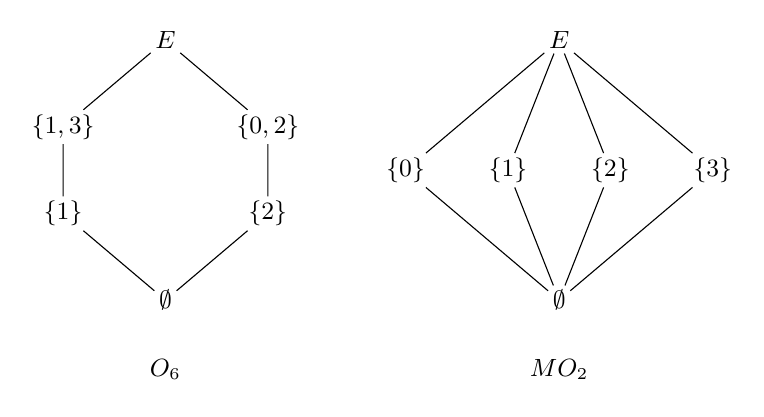
\begin{tikzpicture}[x=1.3cm,y=1.1cm, lab/.style={font=\small, inner sep=1.5pt}]
\begin{scope}
\node[lab] (b) at (0,0) {$\emptyset$};
\node[lab] (x1) at (-1,1) {$\{1\}$};
\node[lab] (x13) at (-1,2) {$\{1,3\}$};
\node[lab] (x2) at (1,1) {$\{2\}$};
\node[lab] (x02) at (1,2) {$\{0,2\}$};
\node[lab] (t) at (0,3) {$E$};
\draw (b) -- (x1) -- (x13) -- (t) -- (x02) -- (x2) -- (b);
\node[font=\small] at (0,-0.8) {$O_6$};
\end{scope}
\begin{scope}[xshift=5cm]
\node[lab] (b) at (0,0) {$\emptyset$};
\foreach \n/\x in {0/-1.5,1/-0.5,2/0.5,3/1.5} {
  \node[lab] (y\n) at (\x,1.5) {$\{\n\}$};
  \draw (b) -- (y\n);
}
\node[lab] (t) at (0,3) {$E$};
\foreach \n in {0,1,2,3} \draw (y\n) -- (t);
\node[font=\small] at (0,-0.8) {$MO_2$};
\end{scope}
\end{tikzpicture}
\caption{Les supports des deux dispositions, ordonnés par l'inclusion. Dans $O_6$, l'orthocomplément échange $\{1\}$ et $\{0,2\}$, $\{2\}$ et $\{1,3\}$ ; dans $MO_2$, il échange $\{0\}$ et $\{1\}$, $\{2\}$ et $\{3\}$. Figure de l'édition. À la page~112, Grothendieck dessine un treillis en perspective, comme un prisme, pour y chercher un contre-exemple, vérifie les compléments et note \q{pas OK !} pour l'un d'eux (\lot{156-9}{6}{112}).}
\label{fig:156-9-spatios}
\end{figure}

\begin{encadre}
\begin{contrexemple}[Réponse à la question de la page 110]
Les supports de $O_6$ sont $\emptyset$, $\{1\}$, $\{2\}$, $\{0,2\}$, $\{1,3\}$ et $E$ ; ceux de $MO_2$ sont $\emptyset$, $\{0\}$, $\{1\}$, $\{2\}$, $\{3\}$ et $E$. Dans les deux cas, l'orthogonal est une involution des supports qui renverse l'inclusion, et $A \cap A^{\perp} = \emptyset$ : ce sont deux spatios finis. Le premier n'est pas orthomodulaire : $\{1\} \subset \{1,3\}$, mais $\{1\} \vee (\complement\{1\} \wedge \{1,3\}) = \{1\}$. Le second est orthomodulaire et n'est pas distributif : $\{0\} \wedge (\{2\} \vee \{3\}) = \{0\}$, tandis que $(\{0\} \wedge \{2\}) \vee (\{0\} \wedge \{3\}) = \emptyset$. Il n'est donc pas une algèbre de Boole.
\end{contrexemple}
\end{encadre}

\begin{proof}
Dans $O_6$, l'orthogonal d'une partie est l'ensemble des voisins communs à tous ses points : $\{1\}^{\perp} = \{0,2\}$ et $\{0,2\}^{\perp} = \{1\}$, $\{2\}^{\perp} = \{1,3\}$ et $\{1,3\}^{\perp} = \{2\}$, tandis que $\{1,2\}^{\perp} = \emptyset$, $\{0\}^{\perp\perp} = \{1\}^{\perp} = \{0,2\}$, $\{3\}^{\perp\perp} = \{1,3\}$ ; la liste des seize parties donne les six supports. Comme $\{0,2\} \cap \{1,3\} = \emptyset$, le reste de $\{1,3\}$ hors de $\{1\}$ est vide. Dans $MO_2$, l'orthogonal de $\{0\}$ est $\{1\}$, et une partie qui contient deux points d'une même paire, ou deux points de paires différentes, a un orthogonal vide ; les supports sont les singletons, le vide et $E$. Pour $b \subset c$ deux supports, ou bien $b = c$, ou bien $b = \emptyset$, ou bien $c = E$ ; dans chaque cas $b \vee (\complement b \wedge c) = c$. Enfin $\{2\} \vee \{3\} = \{2,3\}^{\perp\perp} = \emptyset^{\perp} = E$. En Lean, la liste des supports, la structure de spatios, la loi orthomodulaire pour tous les couples et les deux calculs sont vérifiés par énumération exhaustive dans le noyau.
\end{proof}

\begin{remarque}
Les deux doutes de la page~110 sont fondés, et la troisième question a une réponse négative. Le spatios $O_6$ est l'hexagone de la cote 156-4 : dans le modèle à sept multistrates de la section~\ref{sec:156-4}, les paires disjointes sont celles d'un chemin $a - b - c - d$, qui est la disposition $O_6$, et les parties saturées y sont les mêmes six parties. La première mouture présumait une algèbre de Boole ; l'exemple qui réfute cette présomption réfute aussi la condition plus faible que le chapitre~IX met à sa place. Les deux treillis sont classiques ; la page~110 suggère de chercher parmi les spatios d'un ensemble ordonné muni de la disposition \q{être comparables}, et le prisme de la page~112 n'est pas assez lisible pour qu'on en reconstitue la construction.
\end{remarque}

\subsection*{Transposées qui commutent au complémentaire}

\begin{encadre}
\begin{theoreme}[D'après la page 107, question résolue par l'édition]
Soient $(\Sigma, \leq, \complement)$ et $(\Sigma', \leq, \complement')$ deux ensembles ordonnés munis d'involutions qui renversent l'ordre, $\alpha : \Sigma \to \Sigma'$ et $\beta : \Sigma' \to \Sigma$ deux applications, $\beta$ transposée de $\alpha$ : $\alpha(x) \leq \complement' y$ si et seulement si $x \leq \complement \beta(y)$. Si $\alpha$ et $\beta$ commutent aux complémentaires, alors $\alpha \circ \beta = \mathrm{id}$ et $\beta \circ \alpha = \mathrm{id}$ : ce sont des isomorphismes de spatios inverses l'un de l'autre.
\end{theoreme}
\end{encadre}

\begin{proof}
En remplaçant $y$ par $\complement' y$ dans la définition de la transposée et en utilisant $\beta(\complement' y) = \complement \beta(y)$, on obtient $\alpha(x) \leq y$ si et seulement si $x \leq \beta(y)$ : $\alpha$ est adjoint à gauche de $\beta$. Donc $\alpha\beta(y) \leq y$ et $x \leq \beta\alpha(x)$. Appliquée à $\complement' y$, la première inégalité donne $\alpha\beta(\complement' y) = \complement' \alpha\beta(y) \leq \complement' y$, d'où $y \leq \alpha\beta(y)$ ; appliquée à $\complement x$, la seconde donne $\complement x \leq \beta\alpha(\complement x) = \complement \beta\alpha(x)$, d'où $\beta\alpha(x) \leq x$.
\end{proof}

La question de la page~107 est lue en partie avec doute (\q{Si $\alpha_*$ et $\beta_*$ commutent à $\complement$ [\dots] un iso.\ de spatios, inverses l'un de l'autre ?}, \lot{156-9}{6}{107}). La réponse n'utilise ni les bornes supérieures ni aucune hypothèse booléenne, alors que les équivalences voisines de la page~104, établies pour des parties d'ensembles, passent selon la page~106 par des hypothèses \q{draconiennes} (\lot{156-9}{6}{106}).

Ne sont pas démontrés ici : l'équivalence, au corollaire de la page~108, de la loi orthomodulaire avec la condition sur les familles finies d'éléments deux à deux disjoints (le théorème de Foulis et Holland) ; l'équivalence d'Atmagsupp~1 avec l'orthomodularité pour l'atelier universel d'un spatios ; l'équivalence, établie par les pages~89 à~99, entre les correspondances transposables et les applications qui commutent aux bornes supérieures, que la recherche a retrouvée dans la théorie des concepts formels\pisteresolue{156-9-disposition-correspondences}.
